% Created by tikzDevice version 0.6.1 on 2016-06-13 09:43:08
% !TEX encoding = UTF-8 Unicode
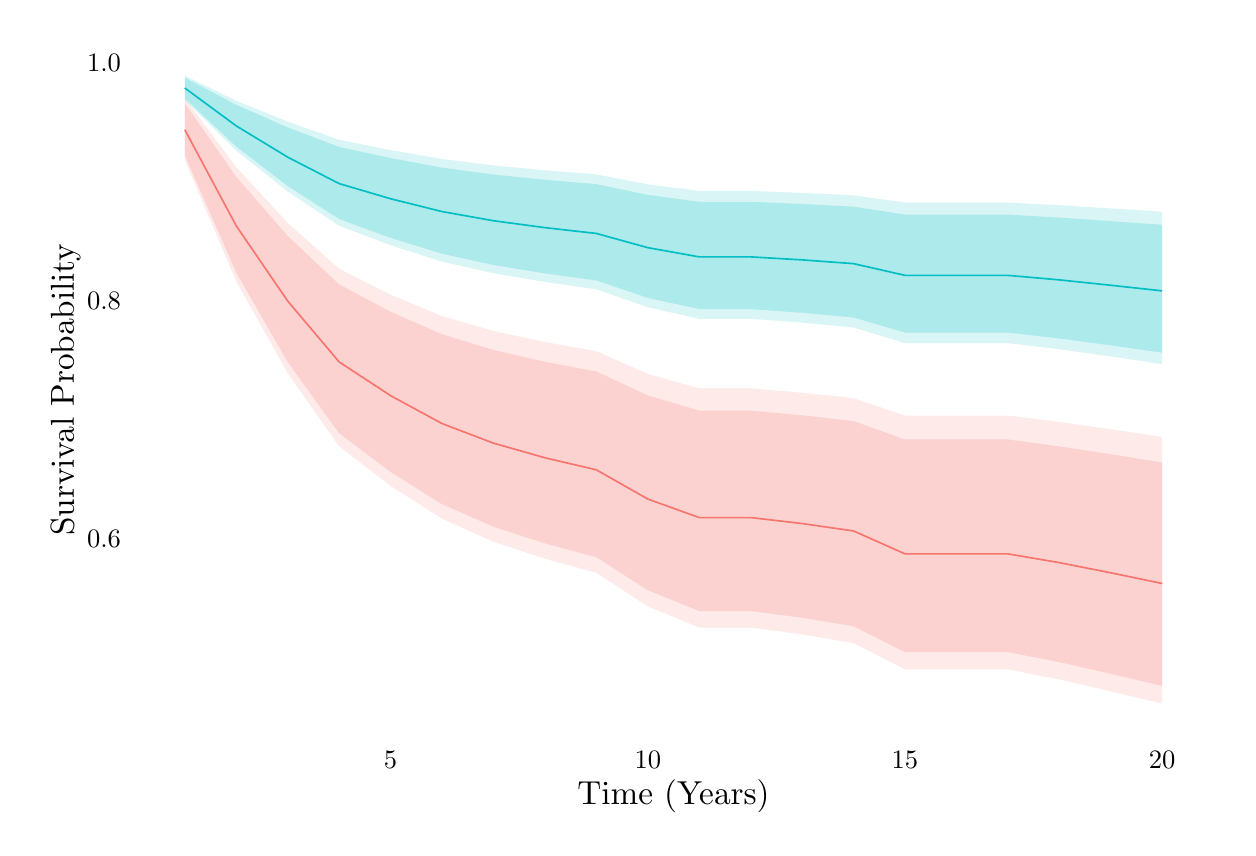
\begin{tikzpicture}[x=1pt,y=1pt]
\definecolor[named]{drawColor}{rgb}{0.00,0.00,0.00}
\definecolor[named]{fillColor}{rgb}{1.00,1.00,1.00}
\fill[color=fillColor,] (0,0) rectangle (433.62,289.08);
\begin{scope}
\path[clip] (  0.00,  0.00) rectangle (433.62,289.08);
\end{scope}
\begin{scope}
\path[clip] (  0.00,  0.00) rectangle (433.62,289.08);
\end{scope}
\begin{scope}
\path[clip] (  0.00,  0.00) rectangle (433.62,289.08);
\end{scope}
\begin{scope}
\path[clip] (  0.00,  0.00) rectangle (433.62,289.08);
\end{scope}
\begin{scope}
\path[clip] (  0.00,  0.00) rectangle (433.62,289.08);
\end{scope}
\begin{scope}
\path[clip] (  0.00,  0.00) rectangle (433.62,289.08);
\end{scope}
\begin{scope}
\path[clip] (  0.00,  0.00) rectangle (433.62,289.08);
\end{scope}
\begin{scope}
\path[clip] (  0.00,  0.00) rectangle (433.62,289.08);
\end{scope}
\begin{scope}
\path[clip] (  0.00,  0.00) rectangle (433.62,289.08);
\end{scope}
\begin{scope}
\path[clip] (  0.00,  0.00) rectangle (433.62,289.08);
\definecolor[named]{drawColor}{rgb}{1.00,1.00,1.00}
\definecolor[named]{fillColor}{rgb}{1.00,1.00,1.00}

\draw[color=drawColor,line width= 0.6pt,line cap=round,line join=round,fill=fillColor,] (  0.00,  0.00) rectangle (433.62,289.08);
\end{scope}
\begin{scope}
\path[clip] (  0.00,  0.00) rectangle (433.62,289.08);
\end{scope}
\begin{scope}
\path[clip] (  0.00,  0.00) rectangle (433.62,289.08);
\end{scope}
\begin{scope}
\path[clip] (  0.00,  0.00) rectangle (433.62,289.08);
\end{scope}
\begin{scope}
\path[clip] ( 39.13, 33.48) rectangle (427.62,283.08);
\definecolor[named]{fillColor}{rgb}{1.00,1.00,1.00}

\draw[fill=fillColor,draw opacity=0.00,] ( 39.13, 33.48) rectangle (427.62,283.08);
\definecolor[named]{drawColor}{rgb}{0.97,0.46,0.43}
\definecolor[named]{fillColor}{rgb}{0.97,0.46,0.43}

\draw[color=drawColor,line width= 0.6pt,line join=round,] ( 56.79,252.18) --
	( 75.38,217.44) --
	( 93.96,190.29) --
	(112.55,168.29) --
	(131.14,156.11) --
	(149.73,146.02) --
	(168.32,138.94) --
	(186.90,133.67) --
	(205.49,129.30) --
	(224.08,118.75) --
	(242.67,112.05) --
	(261.26,112.05) --
	(279.84,109.90) --
	(298.43,107.21) --
	(317.02, 98.94) --
	(335.61, 98.94) --
	(354.20, 98.94) --
	(372.79, 95.77) --
	(391.37, 92.09) --
	(409.96, 88.24);
\definecolor[named]{drawColor}{rgb}{0.00,0.75,0.77}
\definecolor[named]{fillColor}{rgb}{0.00,0.75,0.77}

\draw[color=drawColor,line width= 0.6pt,line join=round,] ( 56.79,267.27) --
	( 75.38,253.58) --
	( 93.96,242.29) --
	(112.55,232.73) --
	(131.14,227.26) --
	(149.73,222.63) --
	(168.32,219.31) --
	(186.90,216.82) --
	(205.49,214.72) --
	(224.08,209.58) --
	(242.67,206.25) --
	(261.26,206.25) --
	(279.84,205.17) --
	(298.43,203.81) --
	(317.02,199.58) --
	(335.61,199.58) --
	(354.20,199.58) --
	(372.79,197.94) --
	(391.37,196.00) --
	(409.96,193.97);
\definecolor[named]{fillColor}{rgb}{0.97,0.46,0.43}

\draw[fill=fillColor,fill opacity=0.15,draw opacity=0.00,] ( 56.79,263.55) --
	( 75.38,238.63) --
	( 93.96,218.49) --
	(112.55,201.93) --
	(131.14,192.55) --
	(149.73,184.85) --
	(168.32,179.47) --
	(186.90,175.46) --
	(205.49,172.13) --
	(224.08,163.94) --
	(242.67,158.74) --
	(261.26,158.74) --
	(279.84,157.15) --
	(298.43,155.17) --
	(317.02,148.92) --
	(335.61,148.92) --
	(354.20,148.92) --
	(372.79,146.59) --
	(391.37,143.97) --
	(409.96,141.17) --
	(409.96, 44.82) --
	(391.37, 49.25) --
	(372.79, 53.56) --
	(354.20, 57.21) --
	(335.61, 57.21) --
	(317.02, 57.21) --
	(298.43, 66.70) --
	(279.84, 69.85) --
	(261.26, 72.33) --
	(242.67, 72.33) --
	(224.08, 79.99) --
	(205.49, 92.11) --
	(186.90, 97.19) --
	(168.32,103.34) --
	(149.73,111.65) --
	(131.14,123.51) --
	(112.55,137.83) --
	( 93.96,164.23) --
	( 75.38,197.41) --
	( 56.79,241.12) --
	cycle;
\definecolor[named]{fillColor}{rgb}{0.00,0.75,0.77}

\draw[fill=fillColor,fill opacity=0.15,draw opacity=0.00,] ( 56.79,271.73) --
	( 75.38,262.67) --
	( 93.96,255.11) --
	(112.55,248.57) --
	(131.14,244.84) --
	(149.73,241.62) --
	(168.32,239.30) --
	(186.90,237.53) --
	(205.49,236.05) --
	(224.08,232.44) --
	(242.67,230.10) --
	(261.26,230.10) --
	(279.84,229.36) --
	(298.43,228.48) --
	(317.02,225.89) --
	(335.61,225.89) --
	(354.20,225.89) --
	(372.79,224.92) --
	(391.37,223.78) --
	(409.96,222.60) --
	(409.96,167.52) --
	(391.37,170.28) --
	(372.79,172.87) --
	(354.20,175.09) --
	(335.61,175.09) --
	(317.02,175.09) --
	(298.43,180.74) --
	(279.84,182.52) --
	(261.26,183.89) --
	(242.67,183.89) --
	(224.08,188.07) --
	(205.49,194.57) --
	(186.90,197.20) --
	(168.32,200.35) --
	(149.73,204.55) --
	(131.14,210.47) --
	(112.55,217.52) --
	( 93.96,229.88) --
	( 75.38,244.68) --
	( 56.79,262.86) --
	cycle;
\definecolor[named]{fillColor}{rgb}{0.97,0.46,0.43}

\draw[fill=fillColor,fill opacity=0.20,draw opacity=0.00,] ( 56.79,261.70) --
	( 75.38,235.14) --
	( 93.96,213.80) --
	(112.55,196.30) --
	(131.14,186.42) --
	(149.73,178.29) --
	(168.32,172.60) --
	(186.90,168.35) --
	(205.49,164.83) --
	(224.08,156.20) --
	(242.67,150.71) --
	(261.26,150.71) --
	(279.84,149.02) --
	(298.43,146.91) --
	(317.02,140.27) --
	(335.61,140.27) --
	(354.20,140.27) --
	(372.79,137.77) --
	(391.37,134.94) --
	(409.96,131.94) --
	(409.96, 51.24) --
	(391.37, 55.60) --
	(372.79, 59.83) --
	(354.20, 63.42) --
	(335.61, 63.42) --
	(317.02, 63.42) --
	(298.43, 72.76) --
	(279.84, 75.85) --
	(261.26, 78.29) --
	(242.67, 78.29) --
	(224.08, 85.82) --
	(205.49, 97.74) --
	(186.90,102.73) --
	(168.32,108.75) --
	(149.73,116.90) --
	(131.14,128.51) --
	(112.55,142.53) --
	( 93.96,168.29) --
	( 75.38,200.55) --
	( 56.79,242.88) --
	cycle;
\definecolor[named]{fillColor}{rgb}{0.00,0.75,0.77}

\draw[fill=fillColor,fill opacity=0.20,draw opacity=0.00,] ( 56.79,271.01) --
	( 75.38,261.19) --
	( 93.96,253.03) --
	(112.55,245.98) --
	(131.14,241.96) --
	(149.73,238.50) --
	(168.32,236.01) --
	(186.90,234.12) --
	(205.49,232.54) --
	(224.08,228.67) --
	(242.67,226.16) --
	(261.26,226.16) --
	(279.84,225.36) --
	(298.43,224.40) --
	(317.02,221.53) --
	(335.61,221.53) --
	(354.20,221.53) --
	(372.79,220.45) --
	(391.37,219.17) --
	(409.96,217.85) --
	(409.96,171.63) --
	(391.37,174.28) --
	(372.79,176.78) --
	(354.20,178.91) --
	(335.61,178.91) --
	(317.02,178.91) --
	(298.43,184.35) --
	(279.84,186.06) --
	(261.26,187.39) --
	(242.67,187.39) --
	(224.08,191.44) --
	(205.49,197.73) --
	(186.90,200.28) --
	(168.32,203.33) --
	(149.73,207.40) --
	(131.14,213.12) --
	(112.55,219.92) --
	( 93.96,231.85) --
	( 75.38,246.10) --
	( 56.79,263.57) --
	cycle;
\end{scope}
\begin{scope}
\path[clip] (  0.00,  0.00) rectangle (433.62,289.08);
\end{scope}
\begin{scope}
\path[clip] (  0.00,  0.00) rectangle (433.62,289.08);
\end{scope}
\begin{scope}
\path[clip] (  0.00,  0.00) rectangle (433.62,289.08);
\end{scope}
\begin{scope}
\path[clip] (  0.00,  0.00) rectangle (433.62,289.08);
\end{scope}
\begin{scope}
\path[clip] (  0.00,  0.00) rectangle (433.62,289.08);
\end{scope}
\begin{scope}
\path[clip] (  0.00,  0.00) rectangle (433.62,289.08);
\definecolor[named]{drawColor}{rgb}{0.00,0.00,0.00}

\node[color=drawColor,anchor=base east,inner sep=0pt, outer sep=0pt, scale=  0.96] at ( 33.73,101.14) {0.6%
};

\node[color=drawColor,anchor=base east,inner sep=0pt, outer sep=0pt, scale=  0.96] at ( 33.73,187.11) {0.8%
};

\node[color=drawColor,anchor=base east,inner sep=0pt, outer sep=0pt, scale=  0.96] at ( 33.73,273.08) {1.0%
};
\end{scope}
\begin{scope}
\path[clip] (  0.00,  0.00) rectangle (433.62,289.08);
\end{scope}
\begin{scope}
\path[clip] (  0.00,  0.00) rectangle (433.62,289.08);
\end{scope}
\begin{scope}
\path[clip] (  0.00,  0.00) rectangle (433.62,289.08);
\end{scope}
\begin{scope}
\path[clip] (  0.00,  0.00) rectangle (433.62,289.08);
\end{scope}
\begin{scope}
\path[clip] (  0.00,  0.00) rectangle (433.62,289.08);
\end{scope}
\begin{scope}
\path[clip] (  0.00,  0.00) rectangle (433.62,289.08);
\end{scope}
\begin{scope}
\path[clip] (  0.00,  0.00) rectangle (433.62,289.08);
\end{scope}
\begin{scope}
\path[clip] (  0.00,  0.00) rectangle (433.62,289.08);
\end{scope}
\begin{scope}
\path[clip] (  0.00,  0.00) rectangle (433.62,289.08);
\end{scope}
\begin{scope}
\path[clip] (  0.00,  0.00) rectangle (433.62,289.08);
\end{scope}
\begin{scope}
\path[clip] (  0.00,  0.00) rectangle (433.62,289.08);
\end{scope}
\begin{scope}
\path[clip] (  0.00,  0.00) rectangle (433.62,289.08);
\definecolor[named]{drawColor}{rgb}{0.00,0.00,0.00}

\node[color=drawColor,anchor=base,inner sep=0pt, outer sep=0pt, scale=  0.96] at (131.14, 21.46) {5%
};

\node[color=drawColor,anchor=base,inner sep=0pt, outer sep=0pt, scale=  0.96] at (224.08, 21.46) {10%
};

\node[color=drawColor,anchor=base,inner sep=0pt, outer sep=0pt, scale=  0.96] at (317.02, 21.46) {15%
};

\node[color=drawColor,anchor=base,inner sep=0pt, outer sep=0pt, scale=  0.96] at (409.96, 21.46) {20%
};
\end{scope}
\begin{scope}
\path[clip] (  0.00,  0.00) rectangle (433.62,289.08);
\end{scope}
\begin{scope}
\path[clip] (  0.00,  0.00) rectangle (433.62,289.08);
\end{scope}
\begin{scope}
\path[clip] (  0.00,  0.00) rectangle (433.62,289.08);
\end{scope}
\begin{scope}
\path[clip] (  0.00,  0.00) rectangle (433.62,289.08);
\definecolor[named]{drawColor}{rgb}{0.00,0.00,0.00}

\node[color=drawColor,anchor=base,inner sep=0pt, outer sep=0pt, scale=  1.20] at (233.37,  8.40) {Time (Years)%
};
\end{scope}
\begin{scope}
\path[clip] (  0.00,  0.00) rectangle (433.62,289.08);
\end{scope}
\begin{scope}
\path[clip] (  0.00,  0.00) rectangle (433.62,289.08);
\definecolor[named]{drawColor}{rgb}{0.00,0.00,0.00}

\node[rotate= 90.00,color=drawColor,anchor=base,inner sep=0pt, outer sep=0pt, scale=  1.20] at ( 16.66,158.28) {Survival Probability%
};
\end{scope}
\begin{scope}
\path[clip] (  0.00,  0.00) rectangle (433.62,289.08);
\end{scope}
\begin{scope}
\path[clip] (  0.00,  0.00) rectangle (433.62,289.08);
\end{scope}
\begin{scope}
\path[clip] (  0.00,  0.00) rectangle (433.62,289.08);
\end{scope}
\begin{scope}
\path[clip] (  0.00,  0.00) rectangle (433.62,289.08);
\end{scope}
\end{tikzpicture}
